\section{Proposed NeST-Com Framework}
\subsection{Next-Scale Representation and Digital Frame}
We transmit $x\in[0,1]^{256\times256\times3}$ using $N$ complex symbols over AWGN,
\begin{equation}
y=s+n,\quad n\sim\mathcal{CN}(0,\sigma^2 I_N),\quad
\mathrm{SNR}=10\log_{10}(E_s/\sigma^2),
\label{eq:channel}
\end{equation}
with nominal $E_s=2$. TX uses the frozen policy for its design SNR; RX uses the actual noise variance for LLRs. Digital constellations have average energy two without per-frame renormalization. A 12-bit profile ID, CRC16, and terminated rate-1/2 convolutional code occupy 68 rotated-BPSK symbols $\{\pm(1+j)\}$. The profile identifies the endpoint and MCS. The remaining $N-68$ symbols carry the LDPC-coded body, with public frame-dependent scrambling after rate matching and inverse scrambling before decoding. Continuous JSCC data are normalized per image to energy two; required side information is paid within $N$.

The frozen VAR tokenizer produces ten residual token maps $q_s$, with side lengths $(1,2,3,4,5,6,8,10,13,16)$ and a 4096-entry codebook~\cite{var}. Write $L_s$ for the number of positions and $C_s$ for codebook lookup, resizing to the full latent grid, and the scale-dependent residual transform. The latent sum $\sum_s C_s(q_s)$ progressively refines a full-field description. Decoder $\Dc$ is adapted on 20\,000 ImageNet training images using MSE plus $0.1$ LPIPS, then frozen. Training mixes continuous, fully quantized, and interpolated prefix-completed latents in proportions 50/25/25\%; the latter use completion from eight source scales (Supplement~S1). The null-class VAR-d16 prior factorizes as
\begin{equation}
p_\theta(q_s\mid q_{<s})=\prod_{i=1}^{L_s}p_\theta(q_{s,i}\mid q_{<s}).
\label{eq:prior}
\end{equation}
Every boundary position has coding probabilities conditioned on the same complete coarse maps. Both terminals reconstruct identical integer CDFs, with total frequency $2^{24}$, for arithmetic coding~\cite{arithmetic}; no unreceived same-scale token is needed.

\begin{figure*}[t]
\centering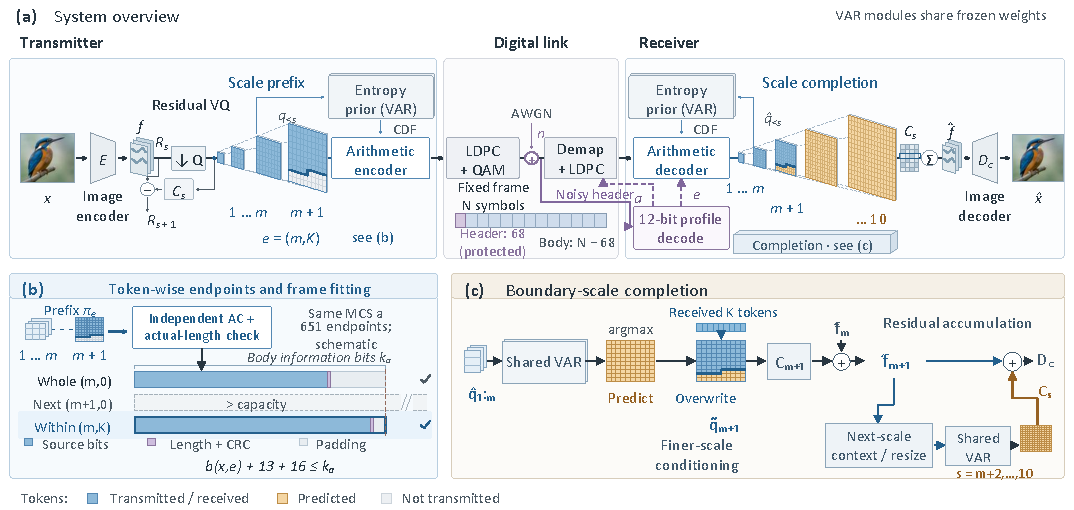
\includegraphics[width=\textwidth]{figure1.pdf}
\caption{NeST-Com. (a) The protected profile specifies the endpoint and MCS; both terminals reconstruct coding probabilities from the shared frozen VAR and known coarse tokens. (b) Independently terminated token-wise prefixes fit the body capacity; bars are schematic. (c) Received boundary tokens overwrite predicted positions. The merged map updates the residual latent and finer-scale context. Unreceived boundary positions retain their coarse-conditioned predictions.}
\label{fig:system}
\end{figure*}

\subsection{Within-Scale Endpoints and Actual-Length Fitting}
An endpoint $e=(m,K)$ retains complete coarse maps and a raster-ordered boundary prefix:
\begin{equation}
\pi_e=(q_1,\ldots,q_m,q_{m+1,1:K}).
\label{eq:prefix}
\end{equation}
The fixed raster order specifies received positions without a mask. WHOLE permits $(m,0)$ for $m=4,\ldots,10$. NeST permits every integer $K=0,\ldots,L_{m+1}-1$ for $m=4,\ldots,9$, together with $(10,0)$: 651 distinct endpoints from 30 through 680 retained tokens. The paid 12-bit profile directory covers the applicable endpoint/MCS combinations. Quarter and Eighth grids are controls, not the main configuration.

For MCS $a=(M,r)$, the coded body has $n_a=(N-68)\log_2M$ bits and information length $k_a=\lfloor rn_a\rfloor$. Its independently terminated arithmetic length $b(x,e)$ must satisfy
\begin{equation}
b(x,e)+29\leq k_a,\qquad \eta(x,e)=\frac{b(x,e)}{k_a-29}.
\label{eq:budget}
\end{equation}
The 29 bits comprise a 13-bit length and CRC16. Unused information positions are zero-padded before 5G NR LDPC coding, rate matching~\cite{nr}, and QAM. Thus $\eta$ is source-bit capacity utilization, not total air-interface efficiency.

Offline calibration fixes a target endpoint and MCS for each budget/SNR by source/reconstruction DINOv2 cosine~\cite{dinov2}. NeST retains these target/MCS choices while refining the available endpoints. Family-specific candidate pools and selection rules are in Supplement~S1. A common scale-wise probability and incremental coding traversal supplies candidates; non-mutating finalization terminates each stream independently, rather than cutting a longer stream. Online, TX holds the MCS fixed, checks endpoints no longer than the target in decreasing token count, and retains the first satisfying~\eqref{eq:budget}. This finds the longest feasible prefix without assuming monotone code lengths or selecting by image quality. If none fits, the frozen $N=1024$ implementation raises an error; this did not occur in the evaluated sources. The $N=512$ implementation instead transmits a paid NULL profile and yields gray.

\ifCLASSOPTIONonecolumn\else\begin{figure*}[t]
\centering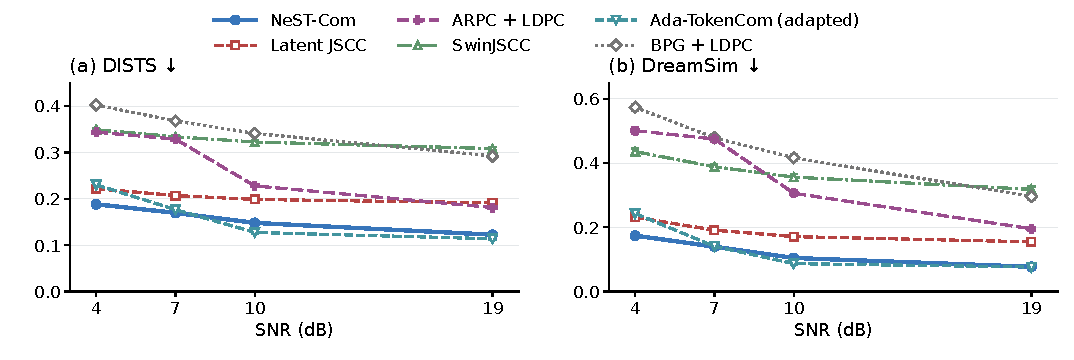
\includegraphics[width=\textwidth]{figure2.pdf}
\caption{Six-system reconstruction on common500 at $N=1024$. Points and bars are equal-source means and pointwise 95\% source-bootstrap intervals after averaging three channel realizations per source, including failures. Ada is the predicted-class, fixed-frame adaptation. Lower DISTS and DreamSim are favorable.}
\label{fig:performance}
\end{figure*}
\fi
\subsection{Prefix-Constrained Reconstruction}
Invalid profile CRC/catalogue, body CRC, declared length, known padding, or arithmetic parsing yields a fixed gray image, as does valid NULL reception. Otherwise, RX decodes the actual prefix using the shared CDFs. It predicts the boundary map by argmax conditioned on complete received maps, then overwrites known positions~\cite{var}:
\begin{equation}
\tilde q_{m+1,i}=\begin{cases}\hat q_{m+1,i},&i\leq K,\\q^{\mathrm{pred}}_{m+1,i},&i>K.\end{cases}
\label{eq:overwrite}
\end{equation}
Received boundary tokens serve two roles: they correct the residual representation and, through the merged boundary map, condition finer-scale prediction. Unreceived boundary positions retain their original coarse-conditioned prediction; there is no same-scale prediction loop. Complete received maps remain unchanged. After generating the finer maps,
\begin{equation}
\hat x=\Dc\!\left(\sum_{s=1}^{10}C_s(\tilde q_s)\right).
\label{eq:reconstruction}
\end{equation}
At the last scale, overwrite only changes the residual contribution.
